\documentclass[12pt,a4paper]{beamer}
\usepackage[utf8x]{inputenc}
\usepackage{ucs}
\usepackage[english]{babel}
%\usepackage[german]{babel}
\usepackage{amsmath}
\usepackage{amsfonts}
\usepackage{amssymb}
\usepackage{alltt}
\author{Michael Haas, haas@cl.uni-heidelberg.de}
\title{Spatial Ontologies}
\subtitle{Seminar: Raum-, Zeit- und Ereignisrepräsentation für die semantische Verarbeitung (Dr. Michael Herweg)}
\date{1-07-2013}
\newcommand{\tuple}[1]{\ensuremath{\left \langle #1 \right \rangle }}
\newcommand{\setof}[1]{\ensuremath{\left \{ #1 \right \}}}

\begin{document}


\begin{frame}
\maketitle
\end{frame}

\begin{frame}{Übersicht}
\begin{itemize}
\item Grundlagen Ontologie
\item Spatial Ontologies
\item Frames of Reference
\item Verfügbare Ontologien
\begin{itemize}
    \item SUMO
    \item DOLCE
    \item ...
\end{itemize}
\item Zusammenfassung 
\item \textbf{Fragen? Zu schnell? Fragen!}
\end{itemize}
\end{frame}


\begin{frame}{Motivationsfragen Ontologie}
 - How do we share knowledge? etc TODO
\end{frame}





\begin{frame}{Definition Ontology}
\begin{quote}
An ontology is an explicit specification of a conceptualization.
\end{quote}
Gruber, 1993
\end{frame}

\begin{frame}{Definition Ontology}
Auf Deutsch: TODO
\end{frame}


%Constructing a view of spatial semantics as an additional layer of ontology in this way brings several advantages crucial
%for adequately capturing the relationship between language use and spatial interpretation. First, it supports the application
%of the full range of methods developed within ontological engineering and applied ontology in order to organize the in-
%formation necessary in ways that conform to a strict and formally specified modeling style [65,67,148]. Second, it provides
%a suitable level of abstraction for dealing effectively with spatial language and for describing what linguistic expressions
%themselves bring to the interpretation process—something that has not been found possible when focusing on linguistic ele-
%ments as isolated terms. And third, it allows the relationship between linguistic expressions and spatial interpretation to be
%recast as a particular case of ontological alignment, or mediation, whereby two or more distinct ontologies are brought into
%a formal relationship [89,100,99,80,98]. Combining these considerations establishes a formally robust and well grounded
%framework from which to consider the full flexibility required for dealing with the mapping between language and space.


\begin{frame}{Spatial Ontology}
\begin{itemize}
\item Ontologie für räumliche Konzepte und Begriffe
\item Unterstützt:
\begin{itemize}
    \item Pfadbeschreibung
    \item Szenenbeschreibung
    \item Navigation
\end{itemize}
\item Einsatz in NLP
\begin{itemize}
    \item Schnittstelle zu GIS
    \item Kontext-Basierte Dienste (??)
    \item Roboter
    \item Generell: Abbildung Raum-Sprache
\end{itemize}
\end{itemize}
\end{frame}


%We propose for this a linguistically-motivated ontology, or ‘linguistic ontology’ for short, that provides a specification of an
%encapsulated layer of ontological information motivated solely by the requirements of linguistically-expressed spatial mean-
%ings. This provides a new layer of organization for capturing the contribution of language to spatial interpretation that is
%free of non-linguistic, contextually-dependent additions. We thereby decompose and modularize the problem of interpreting
%and producing spatial language by ‘stratifying’ three ways: (i) lexicogrammatically, (ii) according to a shallow semantics,
%and (iii) by contextualized specifications—all three of which are formally distinct. The application of ontological engineering
%methods then offers considerable benefits for teasing apart the respective contributions made by these essentially distinct
%knowledge sources.



\begin{frame}{Linguistisch motivierte räumliche Ontologie}
\begin{itemize}
\item Verarbeitung räumlicher Ausdrücke benötigt formalisiertes Wissen über mögliche Ausdrücke
\item Ontologie muss sich aus sprachlicher Evidenz ergeben
\item Formalisierung benötigt systematische Betrachtung sprachlicher Ausdrücke
\item $\to$ Empirisch motiviert
\end{itemize}
\end{frame}


% FOR: Bewegung
\begin{frame}{Frames of Reference}
\begin{itemize}
\item Räumliche Ontologie muss diverse sprachliche Phänomene abbilden
\item Frames of Reference: Welches Bezugssystem ist relevant?
\end{itemize}

Ein Boot ist in einem fließenden Fluss verankert. Bewegt sich das Boot?

\end{frame}

% FOR: intrinsische VS extrinsische orientierung
\begin{frame}{Frames of Reference}

\begin{figure}
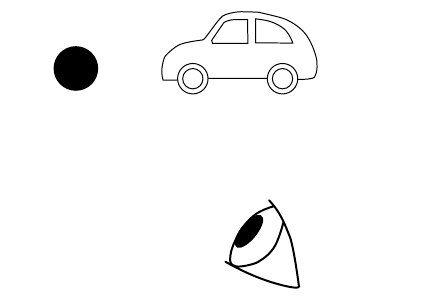
\includegraphics[scale=0.45]{img/levinson_fig_2-1.png}
\caption{Wo ist der Ball? (Figure 2.1, Levinson 2003)}
\end{figure}
\end{frame}


\begin{frame}{Absolute VS relative Frame of Reference}
\begin{itemize}
\item Europäische Sprachen mit relativem Bezugssystem \\
\textit{Is the hot water in the right tap?}
\item Tzeltal mit absolutem Bezugssystem \\
\textit{Is the hot water in the uphill tap?} \\
$\to$ \textit{Is the hot water in the tap that would lie in the uphill southerly direction if I were at home?}
\end{itemize}
\end{frame}



\begin{frame}{Intrinsic Frame of Reference}
\begin{figure}
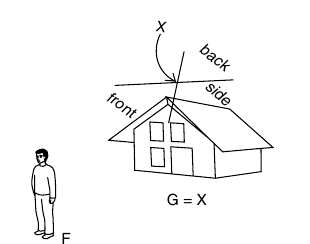
\includegraphics[scale=0.45]{img/levinson_FOR_intrinsic.png}
\caption{Intrinsic FoR (Levinson 2003)}
\end{figure}
\end{frame}

\begin{frame}{Intrinsic Frame of Reference}
\begin{itemize}
\item Im Englischen: Orientierung ergibt sich aus funktionalen Aspekten
\item In Tzeltal: basiert auf Form des Objektes
%\item Oft: Terminologie abgeleitet von Körperteilen\\
%\textit{Am Fuße des Berges}
\item Oft: nur ein Punkt erforderlich; "vorne" ergibt "hinten" \\
$\to$ Nicht in allen Sprachen derartige Opposition verfügbar
\item Suchdomäne unterschiedlich: wie groß ist "vorne"? \\
$\to$ \textit{In front of the church lie the mountains\ldots}
\end{itemize}
\end{frame}


\begin{frame}{Relative Frame of Reference}
\begin{figure}
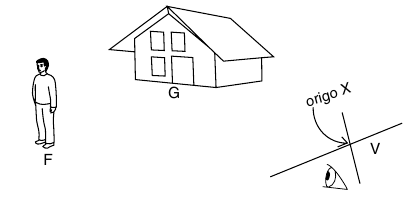
\includegraphics[scale=0.45]{img/levinson_FOR_relative.png}
\caption{Relative FoR (Levinson 2003)}
\end{figure}
\end{frame}

\begin{frame}{Relative Frame of Reference}
\begin{itemize}
\item Koordinationsystem ausgehend von aktuellem Standpunkt V
\item Projiziert auf relatum G
\item Standpunkt muss nicht eigener Ort sein \\
$\to$ \textit{Bill kicked the ball to the left of the goal.}
\item Projektion kann Rotation oder Translation erfahren
% ?? \item Nicht alle Sprachen habe relative FoR ausserhalb intrinsischem Bezug!
\item Ambiguität zwischen intrinsischem und relativem FoR durch überlappende Begriffe \\
$\to$ \textit{to the left of the chair} VS \textit{at the chair's left}
\item Manche Sprachen benutzen "links" etc nur intrinsisch
\item Relative FoR: verzichtbar
\item Kinder lernen projektives "links" erst spät
\item Einige Sprachen benutzen relativen FoR gar nicht
\end{itemize}
\end{frame}


\begin{frame}{Absolute Frame of Reference}
\begin{figure}
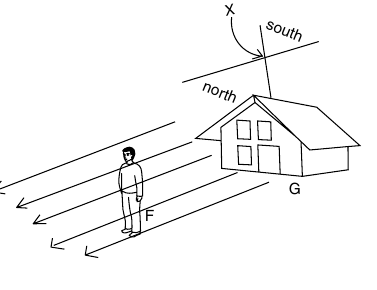
\includegraphics[scale=0.45]{img/levinson_FOR_absolute.png}
\caption{Absolute FoR (Levinson 2003)}
\end{figure}
\end{frame}

\begin{frame}{Absolute Frame of Reference}
\begin{itemize}
\item Kein direkter Bezug zu Orientierung von Betrachter oder Objekt
\item Vertikal: an Schwerkraft orientiert
\item Horizontal: Himmelsrichtungen, landschaftliche Referenzpunkte
\item Sprecher müssen Orientierung behalten
\item Geschätzt ein Drittel aller Sprachen
% Später? \item Unterstützen transitive Inferenz
\end{itemize}
\end{frame}


\begin{frame}{Absolute Frame of Reference: Achsen}
\begin{itemize}
\item Europa: Norden, Süden, Westen, Osten
\item Tenejapa: Norden, Süden, Quer
\item Bali: Achsen gegeben von Monsun und Berg \\
$\to$ Orthogonalität?
\end{itemize}
\end{frame}


\begin{frame}{Drei Frames of Reference}
\begin{itemize}
\item Intrinsic
\item Relative
\item Absolute
\end{itemize}
\end{frame}


\begin{frame}{Frames of Reference: Inferenz und Eigenschaften}
\begin{itemize}
\item Weinheim liegt nördlich von Heidelberg. Darmstadt liegt nördlich von Weinheim. \\
$\to$ Darmstadt liegt nördlich von Heidelberg.
\item Weinheim liegt nördlich von Heidelberg. \\
$\to$ Heidelberg liegt südlich von Weinheim.
\item Jill ist links von Jack. Bill ist links von Jill. \\
$\to$ ?? Bill ist links von Jack ??
\end{itemize}
\end{frame}


\begin{frame}{Transitivity und Converseness}
\begin{figure}
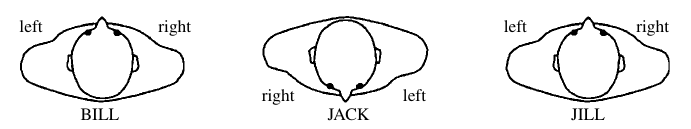
\includegraphics[scale=0.45]{img/levinson_FOR_transitivity.png}
\caption{Transitivity and Converseness (Levinson 2003)}
\end{figure}
Transitivity: Jill ist links von Jack. Bill ist links von Jill. \\
\textbf{!} Bill ist links von jack.\\
Converseness: Jill ist links von Jack. \\
\textbf{!} Jack ist rechts von Jill.
\end{frame}



\begin{frame}{Transitivity und Converseness}
\begin{itemize}
\item Funktioniert für absolute Frame of Reference
\item Funktioniert für relative Frame of Reference bei gleichem Standpunkt
\item Funktioniert \textbf{nicht} für intrinsic Frame of Reference
\end{itemize}
\end{frame}


\begin{frame}{Ontologien}
\begin{itemize}
\item Welche (räumlichen) Ontologien gibt es?
\item Wie berücksichtigen Ontologien die Frames of Reference?
% Müssen Ontologien alle FoR berücksichtigen, oder nur für NLP?
% TODO: Konvertierbarkeit FoR?
\end{itemize}
\end{frame}


\begin{frame}{SUMO}
\begin{itemize}
\item SUMO: Suggested Upper Merged Ontology
\item Kategorien für physische Objekte
\item Mereotopologie
\item Räumliche Relationen
\end{itemize}
\end{frame}

\begin{frame}{SUMO: Object}
\begin{alltt}

(<=> (instance ?PHYS Physical)\\
    (exists (?LOC ?TIME)\\
    (and\\
    (located ?PHYS ?LOC)\\
    (time ?PHYS ?TIME))))\\

\end{alltt}

%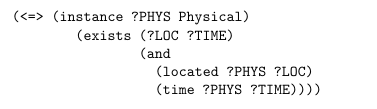
\includegraphics[scale=0.45]{img/d2_object_axiom.png}
%\caption{SUMO Object axiom (Bateman et al, 2004)}
%\end{figure}
%\end{itemize}
\end{frame}




\begin{frame}{SUMO: Region}
\begin{alltt}
(=>
    (instance ?REGION Region)\\
    (exists (?PHYS)\\
    (located ?PHYS ?REGION)))\\
\end{alltt}
\end{frame}



\begin{frame}{SUMO: Region Taxonomy}
%\begin{itemize}
\begin{figure}
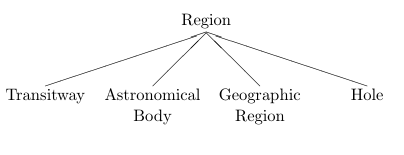
\includegraphics[scale=0.45]{img/d2_region_taxonomy.png}
\caption{SUMO Object axiom (Bateman et al, 2004)}
\end{figure}
%\end{itemize}
\end{frame}

\begin{frame}{SUMO: Position}
\begin{alltt}
PositionalAttribute\\
    Vertical(i)\\
    Horizontal(i)\\
    Above(i)\\
    Below(i)\\
    Adjacent(i)\\
    Left(i)\\
    Right(i)\\
    Near(i)\\
    On(i)\\
\end{alltt}
Subklasse: \textbf{DirectionalAttribute} mit Instanzen North, South, East, West
\end{frame}

\begin{frame}{SUMO: Axiome Position}
\begin{alltt}
(<=>
    (orientation ?OBJ1 ?OBJ2 Vertical)\\
    (orientation ?OBJ2 ?OBJ1 Vertical))\\
(<=>\\
    (orientation ?OBJ1 ?OBJ2 Right) \\
    (orientation ?OBJ2 ?OBJ1 Left))
\end{alltt}
\end{frame}



\begin{frame}{SUMO: Frames of Reference}
\begin{itemize}
\item Positions-Axiome aus wissenschaftlicher Sicht sinnvoll
\item Links immer Gegensatz von rechts?
\item Keine Berücksichtigung unterschiedlicher Frames of Reference
\end{itemize}
\end{frame}


\begin{frame}{OpenCyc}
\begin{quote}
The OpenCyc Platform is your gateway to the full power of Cyc, the world's largest and most complete general knowledge base and commonsense reasoning engine. \footnote{http://www.cyc.com/platform/opencyc Accessed 2013-06-30}
\end{quote}
\begin{figure}
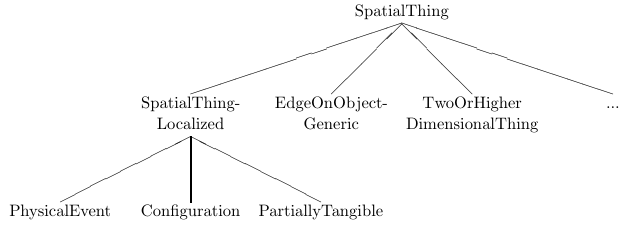
\includegraphics[scale=0.45]{img/d2_opencyc_SpatialThing_taxonomy.png}
\caption{OpenCyc SpatialThing taxonomy (Bateman et al, 2004)}
\end{figure}
\end{frame}

\begin{frame}{OpenCyc: Seiten von Objekten }
\begin{figure}
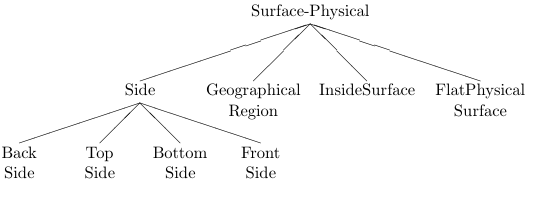
\includegraphics[scale=0.45]{img/d2_opencyc_sides_of_objects.png}
\caption{OpenCyc Sides of objects (Bateman et al, 2004)}
\end{figure}
\end{frame}

\begin{frame}{OpenCyc: Spatial Relations}
\begin{alltt}
near[NaivePhysicsVocabularyMt]:\\
    inFrontOf-Generally\\
    behind-Generally\\
    alignedAlong\\
    hasPortalToRegion\\
    movesWith\\
    stuckTo\\
    spatiallyIntersects\\
    touches\\
\end{alltt}

\end{frame}

%Does inFrontOf-Generally presuppose Side surface?


\begin{frame}{OpenCyc: Orientierung \& Richtung}
\begin{itemize}
\item Orientierung\\
\begin{alltt}
    HorizontalOrientation\\
    VerticalOrientation\\
    UpsideDown\\
    RightSideUp
\end{alltt}
\item Richtung
\begin{alltt}
    Up-Generally\\
    Up-Directly\\
    Down-Generally\\
    Down-Directly\\
    VerticalDirection\\
    HorizontalDirection
\end{alltt}
\end{itemize}
\end{frame}



\begin{frame}{OpenCyc: Geographische Richtung}
\begin{alltt}
    North-Generally\\
    North-Directly\\
    South-Directly\\
    ...\\
    East-Directly
\end{alltt}
\end{frame}


\begin{frame}{OpenCyc: Issues}
\begin{itemize}
\item Keine Beachtung von Frames of Reference
\item Reflektiert teils Besonderheiten des Englischen\\
$\to$ \textit{in-Floating} - Bewegung oder Attribut?
\end{itemize}
\end{frame}



\begin{frame}{GUM: Generalized Upper Model}
\begin{itemize}
\item Räumliche Erweiterung von GUM: basiert rein auf linguistischer Evidenz
\item Keine Festlegung auf Raumstruktur oder Interpretation
\end{itemize}
\end{frame}


\begin{frame}{GUM: Beispiel}
To the left of the computer is a USB drive.

\begin{figure}
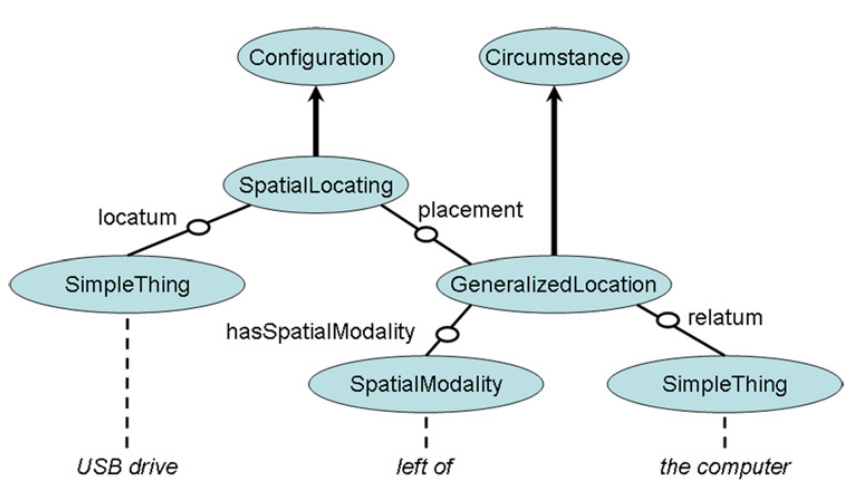
\includegraphics[scale=0.45]{img/2010_fig3.png}
\caption{GUM Representation(Bateman et al, 2010)}
\end{figure}
\end{frame}


\begin{frame}{GUM: Beispiel}
To the left of the computer is a USB drive.

\begin{figure}
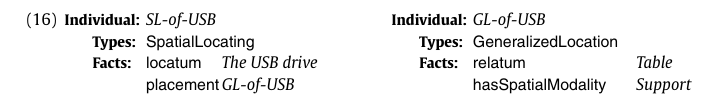
\includegraphics[scale=0.45]{img/2010_gl_of_usb.png}
\caption{GUM Representation(Bateman et al, 2010)}
\end{figure}
\end{frame}


\begin{frame}{GUM: Bewegung, Orientierung ohne Zustandsänderung}
$$ NonAffectingOrienting  $$
$$ NonAffectingMotion \equiv NonAffectingDirectedMotion$$ 
$$\sqcup NonAffectingOrientationChange $$
$$\sqcup NonAffectingSimpleMotion$$
\begin{itemize}
\item \textbf{NonAffectingOrienting}: "We are facing the table"
\item \textbf{NonAffectingSimpleMotion}:  "I ran", "The ball rolls"
\item \textbf{NonAffectingDirectedMotion}: "He walks forward"
\item \textbf{NonAffectingOrientationChange}: "He turned around"
\end{itemize}
\end{frame}


\begin{frame}{GUM: Bewegung mit Zustandsänderung}
Dynamische Prozesse: "He puts the USB drive on the table"
$$AffectingAction \equiv DoingAndHappening \sqcap \exists actee.SimpleThing$$
$$AffectingSpatialAction$$
\begin{figure}
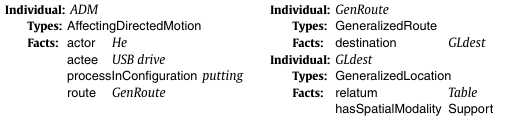
\includegraphics[scale=0.7]{img/2010_puts_usb_on_table.png}
\caption{GUM Representation(Bateman et al, 2010)}
\end{figure}
\end{frame}

\begin{frame}{GUM: Spatial Modalities}
$  SpatialModality \equiv SpatialDistanceModality \sqcup FunctionalSpatialModality \sqcup RelativeSpatialModality $
\begin{itemize}
\item \textbf{SpatialModality} füllt \textbf{hasSpatialModality} Relation in \textbf{GeneralizedLocations}
\begin{itemize}
    \item Statisch: zwischen \textbf{locatum} und \textbf{relatum}
    \item Dynamisch: zwischen \textbf{actor/actee} und \textbf{relatum}
\end{itemize}
\item Beispiele: Support, Proximal, Left-Of
\item Extrema: \textbf{extremePositionOnAxis}, \textbf{extremeDistancePosition} \\
$\to$ "the leftmost", "the closest"
\end{itemize}
\end{frame}

\begin{frame}{GUM: Spatial Modalities}
\begin{itemize}
\item Winkel und Distanzen: \textbf{quantitativeAngleExtent}, \textbf{quantitativeDistanceExtent} \\
$\to$ "They turn around 180 degrees"
\item Qualitativ: \textbf{qualitativeAngleExtent}, \textbf{qualitativeDistanceExtent} \\
$\to$ "Turn a bit further to your right"
\end{itemize}
\end{frame}


\begin{frame}{GUM: Relative Aspekte \& Projektionen}
\begin{itemize}
\item Subklasse \textbf{RelativeSpatialModality}
\item \textbf{HorizontalProjection}, \textbf{VerticalProjection} mit Subklassen \\
\item \textit{In the front of the car} \\
$\to$ \textbf{FrontProjection} unterstützt externe und interne Lesart durch Subsumption
\begin{itemize}
    \item Extern: \textbf{Disjointness} und \textbf{Proximal}
    \item Intern: \textbf{Parthood}
\end{itemize}
\end{itemize}
\end{frame}



\begin{frame}{GUM: Frames of Reference}
\begin{itemize}
\item Frames of Reference realisiert über \textbf{RelativeSpatialModality}
\item Repräsentation verschiedener Lesarten unterstützt \\
$\to$ Entscheidung fällt außerhalb Ontologie über Kontextualisierung
% TODO: ist das so? Oder ist es so zu verstehen, dass Half-Planes bevorzugte Theorie sind?
\item Theorie hinter \textbf{LeftProjection}, \textbf{RightProjection}: Vektoren oder Ebenen? \\
$\to$ Modular, nicht festgelegt \\
$\to$ Inferenz-Regeln nicht festgelegt
\end{itemize}
\end{frame}

\begin{frame}{GUM: Zusammenfassung}
\begin{itemize}
\item Ontologie: formalisierte Grundlage für Wissensdarstellung und -weitergabe
\item Strikt auf Basis linguistischer Daten erstellt
\item Bildet räumliche Phänomene ab
\item Keine Entscheidung für zugrundeliegende Repräsentation
\item Frames of Reference berücksichtigt
\item Kontext benötigt für Frames of Reference
\end{itemize}
\end{frame}




%particularly, cognitive modelling, artificial intelligence, geographic information systems (GIS),
%and the like. The role of an ontology in this area is as it is in all domains and as was introduced
%in our baseline ontology deliverable D1: that is, (i) to set out a consistent and well-specified
%general modelling scheme which is free of contradiction and from which follows a set of generic
%properties that necessarily hold over the entities covered and, (ii) to support problem solving
%and inference within the domain of concern.



%\begin{frame}{CMSM for Sentiment Analysis: Eval Results}
%\begin{figure}
%\includegraphics[scale=0.45]{cmsm_for_se_table3.png}
%\caption{Yessenalina \&  Cardie (2011)}
%\end{figure}

%\end{frame}


\begin{frame}[allowframebreaks]{References}
\begin{thebibliography}{-}
% APA
\bibitem{bateman2010} Bateman, J. A., Hois, J., Ross, R., \& Tenbrink, T. (2010). A linguistic ontology of space for natural language processing. Artificial Intelligence, 174(14), 1027-1071.
\bibitem{bateman2004} Bateman, J., \& Farrar, S. (2004). Spatial ontology baseline. Collaborative Research Center for Spatial Cognition. I1-[OntoSpace] D2
\bibitem{gruber1993} Thomas R. Gruber. A Translation Approach to Portable Ontology Specifications. Knowledge Acquisition, 5(2):199-220, 1993.
\bibitem{levinson2003} Levinson, S. C. (2003). Space in language and cognition: Explorations in cognitive diversity (Vol. 5). Cambridge University Press.
\end{thebibliography}
\end{frame}
\end{document}

